\documentclass[14pt]{beamer}
\title{WEB :: JavaScript}
\author[TS]{TalentSprint}
\institute[L\&D]{Licensed To Skill}
\usefonttheme{serif}
\usecolortheme{orchid}
\usepackage{bookman}
\usepackage{multirow}
\usepackage{hyperref}
\usepackage[T1]{fontenc}
\usepackage{graphicx}
\usepackage{listings}
\graphicspath{{../Images/}}
\usepackage[tikz]{bclogo}
\usepackage{soul}
 \definecolor{light-gray}{gray}{0.80}
 \usepackage{color}
\beamertemplateballitem
\usebackgroundtemplate{
\includegraphics[width=\paperwidth]{TS-XP-Logo.jpg}}
\lstset{language=html, numbers=left, numbers=none, basicstyle=\footnotesize, numberstyle=\tiny,  numbersep=10pt, showstringspaces=false, breaklines=true,keepspaces=true, columns=flexible}
\begin{document}

\begin{frame}
  \titlepage
\end{frame}

\begin{frame}{Learning Objectives}
The content in this presentation is aimed at teaching  learners to:
  \begin{itemize}
  \item Describe Java Script as a scripting language 
  \item List the advantage of Java Script  
  \item Explain fundamental elements of Java Script 
  \item Define functions
  \item Deploy event driven code
  \end{itemize}
\end{frame}

\begin{frame}{JavaScript}
What is Java Script?
\begin{itemize}
 \item Is a scripting language produced by Netscape for use within HTML  Web pages.
 \item Loosely based language and it is built into all the major modern browsers.
 \item Lightweight, interpreted programming language
 \item Open and cross-platform
\end{itemize}
\end{frame}

\begin{frame}{JavaScript}
\textbf{Why Java Script?}

\vspace{1pc}
To overcome HTML Problems:

\vspace{1pc}
\begin{minipage}{1.5cm}

\includegraphics[scale=.25]{javascript-html.png}
\end{minipage}
\quad
\begin{minipage}{7.5cm}
\begin{itemize}
 \item HTML cannot validate the data at client-side
 \item HTML is static, it cannot react to the events
\end{itemize}
\end{minipage}
\end{frame}

\begin{frame}{JavaScript}
Advantages of Java Script
\begin{itemize}
 \item Provides HTML designers a programming tool.
 \item Can reacts to the events.
 \item Validates the data at client-side.
 \item Can read and change the content of an HTML element.
\end{itemize}
\end{frame}

\begin{frame}[fragile]{JavaScript}
\begin{block}{Syntax}
\begin{lstlisting}
<html>
    <head>
        <script type = ``text/javascript''>
            document.write(``<p>'' + Date() + ``</p>'');
        </script>
    </head>
    <body>
        <h1> My First Web Page </h1>
    </body>
</html> 
\end{lstlisting}
\end{block}
\end{frame}

\begin{frame}[fragile]{JavaScript}
\begin{lstlisting}
<script type = ``text/javascript''>
    document.write(``<p>'' + Date() + ``</p>'');
</script>
\end{lstlisting}
\lstinline!<script>! Tag Attributes: language, type
\end{frame}

\begin{frame}[fragile]{JavaScript}
First Java Script
\begin{block}{}
\begin{lstlisting}
<html>
  <body>
      <script language = ``javascript'' type = ``text/javascript''>
          document.write(``Hello World!'')
      </script>
  </body>
</html>
\end{lstlisting}
\end{block}
\begin{block}{Note}
JavaScript ignores spaces, tabs, and newlines that appear in JavaScript programs.
\end{block}
\end{frame}

\begin{frame}[fragile]{JavaScript}
Semicolons
\begin{itemize}
 \item Statements in JavaScript are generally followed by a semicolon character, just as they are in C, C++, and Java.
 \item However, Javascript, allows you to omit this semicolon if your statements are each placed on a separate line.
\end{itemize}
\begin{block}{code without semicolons:}
\begin{lstlisting}
<script language = ``javascript'' type = ``text/javascript''>
    var1 = 10
    var2 = 20
</script>
\end{lstlisting}
\end{block}
\end{frame}

\begin{frame}[fragile]{JavaScript}
\textbf{Semicolons}

\vspace{1pc}
Semicolons are required when formatted in a single line.
\begin{block}{Example}
\begin{lstlisting}
<script language = ``javascript'' type = ``text/javascript''>
    var1 = 10; var2 = 20;
</script>
\end{lstlisting}
\end{block}
It is a good programming practice to use semicolons.
\end{frame}

\begin{frame}{JavaScript}
Case Sensitivity
\small
\begin{itemize}
 \item JavaScript is a case-sensitive language.
 \item Language keywords, variables, function names, and any other identifiers must always be typed with a consistent capitalization of letters.
 \item For example 
 
 Identifier: \em{Time} and \emph{TIME} will have different meanings in JavaScript.
\end{itemize}
\begin{block}{Note}
Care should be taken while writing your variable and function names in JavaScript.
\end{block}
\end{frame}

\begin{frame}{JavaScript}
Comments
\begin{itemize}
 \item Any text before a // and the end of a line is treated as a comment and is ignored by JavaScript. This is for single line comment.
 \item Any text between the characters /* and */ is treated as a comment. This is for multiple lines comments.
\end{itemize}
\end{frame}

\begin{frame}{JavaScript}
JavaScript code can be placed anywhere in an HTML document.

\vspace{1pc}
\colorbox{light-gray}{
\begin{minipage}{10cm}
Script in \lstinline!<head>...</head!> section. 

Script in \lstinline!<body>...</body>! section.

Script in \lstinline!<body>...</body>! and \lstinline!<head>...</head>! sections.

Script in and external file and then include in \lstinline!<head>...</head>! section.
\end{minipage}}
\begin{block}{Note}
The preferred way is to include it in the \lstinline!<head> ... </head>! section.
\end{block}
\end{frame}

\begin{frame}{JavaScript}
\textbf{Java Script Data Types}

\vspace{1pc}
Three primitive data types:
\begin{description}
 \item [Numbers] 123, 120.50 etc.
 
 Example: var num = 2534;
 \item [Strings] ``This text string'' etc.

 Exapmle: var strString = ``This is a string'';
 \item [Boolean] true or false 
 
 Example: var isMarried = true;
\end{description}
\end{frame}

\begin{frame}{JavaScript}
Java Script Data Types

\begin{block}{Note}
 JavaScript is a loosely typed language, the declaration for a string variable, a number and a boolean is same. But it differentiates a string variable, a number and a boolean from the literal value assigned to it and the context of its use.
\end{block}
\end{frame}

\begin{frame}{JavaScript}
Java Script Variables
\begin{figure}[H]
\centering
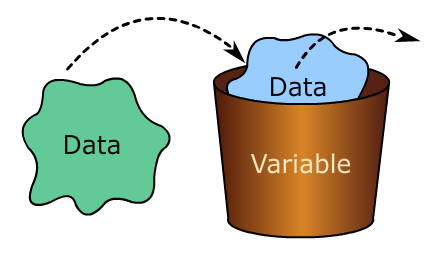
\includegraphics[scale=.25]{js-variables.png}
\end{figure}
Variables can be thought of as named containers. You can place data into these containers and then refer to the data simply by naming the container.
\end{frame}

\begin{frame}[fragile]{JavaScript}
Java Script Variables

\vspace{1pc}
Before you use a variable in a JavaScript program, you must declare it. Variables are declared with the var keyword.
\begin{block}{}
\begin{lstlisting}
<script type = ``text/javascript''>
    var money;
    var name;
</script>
\end{lstlisting}
\end{block}
\end{frame}

\begin{frame}{JavaScript}
\textbf{Java Script Variable Scope}

\vspace{1pc}
The scope of a variable is the region of your program in which it is defined. JavaScript variable will have only two scopes.
\begin{description}
 \item [Global Variables] A global variable has global scope which means it can be accessed any where in a JavaScript code.
\end{description}
\end{frame}

\begin{frame}{JavaScript}
\textbf{Java Script Variable Scope}

\vspace{1pc}
\begin{description}
 \item [Local Variables] A local variable will be visible only within a function where it is defined.
\end{description}
\begin{bclogo}[couleur=blue!5, arrondi=0.3, logo=\bccrayon]{Note}
Function parameters are always local to that function.
\end{bclogo}
\end{frame}

\begin{frame}{JavaScript}
\textbf{JavaScript Variable Names}

\vspace{1pc}
Rules for naming JavaScript variables:
\begin{itemize}
 \item You should not use any of the JavaScript reserved keyword as variable name.
 
 Example: Break or Boolean variable names are not valid as variable names.
 \item Variable names are case-sensitive. 
 
 Example, Name and name are two different variables.
\end{itemize}
\end{frame}

\begin{frame}{JavaScript}
\textbf{JavaScript Variable Names}
\begin{itemize}
 \item Variable names should not start with numeral (0-9). They must begin with a letter or the underscore character.
  
  Example: 123test is an invalid variable name but \_123test is a valid one.
\end{itemize}
\end{frame}

\begin{frame}{JavaScript}
\textbf{Java Script Reserved Words}
\def\arraystretch{1.2}
\begin{center}
\begin{tabular}{l l l l l}
break & case & catch & continue & do \\

default & delete & else & finally & for \\

function & if & in & new & return \\

switch & this & throw & try & typeof \\

var & void & while & & \\

\end{tabular}
\end{center}
Reserve words cannot be used as JavaScript variables, functions, methods, loop labels, or any object names as they have some special meaning.
\end{frame}

\begin{frame}{JavaScript}
What are Operators?
\begin{itemize}
 \item An operator is a symbol that is used to perform an operation.
       
       + - * / \% \mbox{-}\mbox{-} \&\& >

 \item Operators generally work on variables or constants.
 
 \colorbox{orange}{Variables} $\leftarrow$ \colorbox{light-gray}{Operators} $\rightarrow$ \colorbox{green}{Constants}
\end{itemize}

\end{frame}

\begin{frame}{JavaScript}
JavaScript Operators

\vspace{1pc}
\begin{description}
 \item [Arithmetic Operators] +, -, *, /, \%, ++, \mbox{-}\mbox{-}
 \item [Comparison Operators] ==, !=, >, <, >=, <= 
 \item [Logical Operators] \&\&, ||, ! 
 \item [Assignment Operators] =, +=, -+, *=, /=
 \item [Miscellaneous Opertors] Conditional Operator (?)
\end{description}
\end{frame}

\begin{frame}{JavaScript}
Why Conditional Statements?

\vspace{1pc}
Very often, in our programs we will get a situation where in we have to execute some statements depending on some condition. 
\begin{block}{Example}
\begin{minipage}{2cm}
\begin{figure}[H]
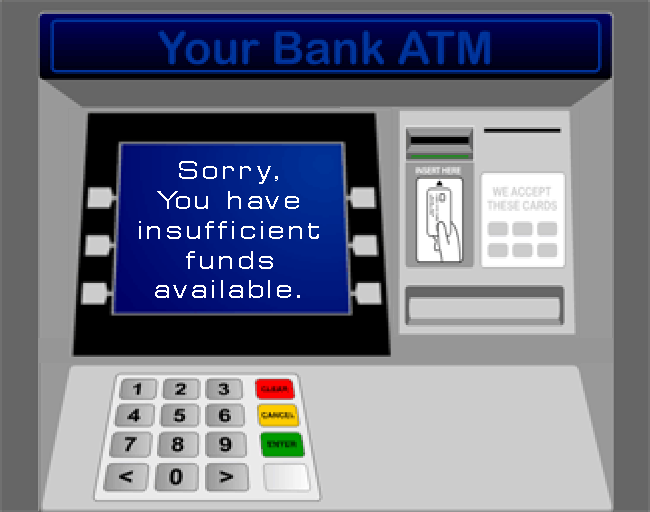
\includegraphics[scale=.1]{conditional-statements.png}
\end{figure}
\end{minipage}
\quad
\begin{minipage}{8cm}
\small
Customer wants to withdraw Rs:5000

Balance availabel Rs:4000

ATM must display: Insufficient Funds
\end{minipage}
\end{block}
For above situations we use conditional statements like if, if-else.
\end{frame}

\begin{frame}[fragile]{JavaScript}
\textbf{Conditional Statements - Flow Control Structures}

\vspace{1pc}
\begin{block}{if - Statement: Syntax}
\begin{lstlisting}[language=java]
if (expression) {
   Statement(s); // executed if expression is true
}
\end{lstlisting}
\end{block}
\end{frame}

\begin{frame}[fragile]{JavaScript}
\textbf{Conditional Statements - Flow Control Structures}

\vspace{1pc}
\begin{block}{if else - Statement: Syntax}
\begin{lstlisting}[language=java]
if (expression) {
    Statement(s); // executed if expression is true
} else {
    Statement(s); // executed if expression is false
}
\end{lstlisting}
\end{block}
\end{frame}

\begin{frame}[fragile]{JavaScript}
\begin{block}{Switch Statement - Syntax}
\begin{lstlisting}[language=java]
switch (expression) {
    case condition 1: 
        statement(s);
        break;
    case condition 2: 
        statement(s);
        break;
    case condition n: 
        statement(s);
        break;
    default: 
        statement(s);
}
\end{lstlisting}
\end{block}
\end{frame}

\begin{frame}[fragile]{JavaScript}
\textbf{Conditional Statements - Looping Control Structures}

\vspace{1pc}
\begin{block}{while - Syntax}
\begin{lstlisting}[language=java]
while (expression) {
    Statement(s); // executed if expression is true
}
\end{lstlisting}
\end{block}
\end{frame}

\begin{frame}[fragile]{JavaScript}
\textbf{Conditional Statements - Looping Control Structures}

\vspace{1pc}
\begin{block}{do..while - Syntax}
\begin{lstlisting}[language=java]
do {
    Statement(s); // to be executed;
} while (expression);
\end{lstlisting}
\end{block}
\end{frame}

\begin{frame}[fragile]{JavaScript}
\textbf{Conditional Statements - Looping Control Structures}

\vspace{1pc}
\begin{block}{for - Syntax}
\begin{lstlisting}[language=java]
for (initialization; test condition; iteration statement) {
     Statement(s); // to be executed if test condition is true
}
\end{lstlisting}
\end{block}

\begin{block}{Advanced `for' - Syntax}
\begin{lstlisting}[language=java]
for (variablename in object) {
    statement or block to execute
}
\end{lstlisting}
\end{block}
\end{frame}

\begin{frame}[fragile]{JavaScript}
\textbf{How to define a function?}

\vspace{1pc}
The most common way to define a function in JavaScript is by using the function keyword, followed by a unique function name, a list of parameters (that might be empty), and a statement block surrounded by curly braces.
\end{frame}

\begin{frame}[fragile]{JavaScript}
\begin{block}{Function - Syntax}
\begin{lstlisting}
<script type = ``text/javascript''>
    function functionname(parameter-list) {
        // statements
    }
</script>
\end{lstlisting}
\end{block}

\begin{block}{Syntax for calling a function}
\begin{lstlisting}
<script type = ``text/javascript''>
    sayHello();
</script>
\end{lstlisting}
\end{block}
\end{frame}

\begin{frame}{JavaScript}
\textbf{Dialog Boxes}

\begin{description}
 \item [Alert Dialog Box] Used to give a warning message to the users
\end{description}
\begin{block}{}
\lstinline!alert(``Warning Message'');!
\end{block}

\begin{figure}[H]
 \centering
 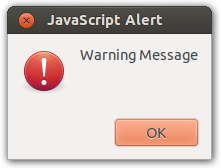
\includegraphics[scale=.4]{alert-box.png}
\end{figure}
\end{frame}

\begin{frame}{JavaScript}
\begin{description}
 \item [Confirmation Dialog Box]\
\end{description} 
 \begin{itemize}
 \item Used to take user's consent on any option. 
 \item Displays a dialog box with two buttons: OK and Cancel.
\end{itemize}
\begin{block}{}
\lstinline!confirm(``Do you want to continue ?'');!
\end{block}
\begin{figure}[H]
\centering
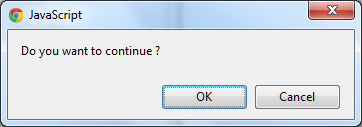
\includegraphics[scale=.4]{conform-box.png}
\end{figure}
\end{frame}

\begin{frame}{JavaScript}
\begin{description}
 \item [Prompt Dialog Box] Prompts the user for a single input
\end{description}
\begin{block}{}
\lstinline!var input = prompt(``Enter your name : '', ``your name here'');!
\end{block}
\begin{figure}[H]
\centering
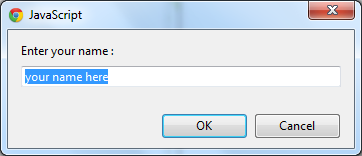
\includegraphics[scale=.4]{prompt-box.png}
\end{figure}
\end{frame}

\begin{frame}{JavaScript}
\textbf{Page Printing}

\vspace{1pc}
The JavaScript print function \textbf{window.print()} will print the current web page when executed.

\begin{block}{}
\lstinline!<input type = ``button'' value = ``Print'' onclick = ``window.print()''/>!
\end{block}
\end{frame}

\begin{frame}{JavaScript}
\textbf{Page Redirection}

\vspace{1pc}
Redirects your site visitors to a new page.
\begin{block}{}
\lstinline!window.location = ``http://www.newlocation.com'';!
\end{block}
\end{frame}
















\begin{frame}{JavaScript}
 \begin{figure}[H]
    
\includegraphics[scale=.3]{qa.png}   
   \end{figure}
\end{frame}

\end{document}
